\documentclass[tikz,border=5mm]{standalone}
\usepackage{amsmath}

% TikZ settings
\tikzset{
    dot/.style={circle, fill, inner sep=1.5pt},
    edge/.style={thick},
}

\begin{document}
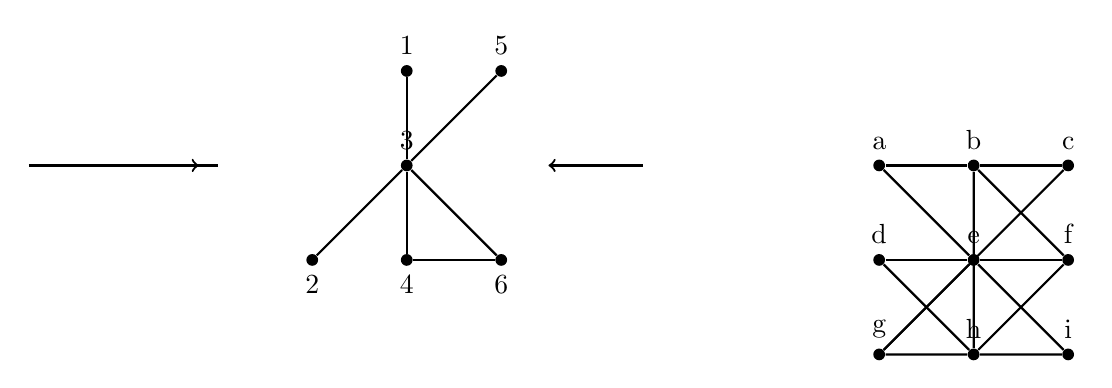
\begin{tikzpicture}[scale=1.2]

% Leftmost part: Horizontal arrow
\draw[edge] (-4,0) -- (-2,0);
\draw[edge, ->] (-3.8,0) -- (-2.2,0);

% Middle part: Graph with labeled vertices
\begin{scope}[shift={(0,0)}]
    % Define vertices
    \node[dot,label=above:$1$] (v1) at (0,1) {};
    \node[dot,label=below:$2$] (v2) at (-1,-1) {};
    \node[dot,label=above:$3$] (v3) at (0,0) {};
    \node[dot,label=below:$4$] (v4) at (0,-1) {};
    \node[dot,label=above:$5$] (v5) at (1,1) {};
    \node[dot,label=below:$6$] (v6) at (1,-1) {};

    % Draw edges
    \draw[edge] (v1) -- (v3);
    \draw[edge] (v2) -- (v3);
    \draw[edge] (v3) -- (v4);
    \draw[edge] (v4) -- (v6);
    \draw[edge] (v5) -- (v3);
    \draw[edge] (v3) -- (v6);

    % Arrow pointing to the right
    \draw[edge, <-] (1.5,0) -- (2.5,0);
\end{scope}

% Rightmost part: Complex graph
\begin{scope}[shift={(5,0)}]
    % Define vertices
    \foreach \i/\j/\k [count=\c] in {
        0/0/a, 1/0/b, 2/0/c,
        0/-1/d, 1/-1/e, 2/-1/f,
        0/-2/g, 1/-2/h, 2/-2/i
    } {
        \node[dot,label=\k] (v\c) at (\i,\j) {};
    }

    % Draw edges
    \draw[edge] (v1) -- (v2); \draw[edge] (v2) -- (v3);
    \draw[edge] (v4) -- (v5); \draw[edge] (v5) -- (v6);
    \draw[edge] (v7) -- (v8); \draw[edge] (v8) -- (v9);

    \draw[edge] (v1) -- (v5); \draw[edge] (v2) -- (v6);
    \draw[edge] (v4) -- (v8); \draw[edge] (v5) -- (v9);
    \draw[edge] (v7) -- (v3); \draw[edge] (v8) -- (v2);

    \draw[edge] (v7) -- (v5); \draw[edge] (v8) -- (v6);
\end{scope}

\end{tikzpicture}
\end{document}